%\documentclass[12pt,a4paper,twosides]{article}
\documentclass[12pt,a4paper,oneside]{article}

\newcommand{\Ham}{\mathcal{H}}
\newcommand{\Kam}{\mathcal{K}}
\newcommand{\Aam}{\mathcal{A}}
\newcommand{\Bam}{\mathcal{B}}
\newcommand{\crochet}[2]{\left\lbrace #1,#2 \right\rbrace }
\newcommand{\fat}[1]{$\displaystyle{#1}$}
\newcommand{\drond}[2]{\frac{\partial #1}{\partial #2}}
\newcommand{\vect}[1]{\mathbf{\boldsymbol{#1}}}
\newcommand{\accolade}{\phantom{\frac{1}{1}\!\!\!\!\!}}
\newcommand{\barre}[1]{\overline{#1}}
\newcommand{\jz}[1]{{#1}_j^{(0)}}
\newcommand{\pp}{\left(p+1\right)}
\newcommand{\R}{\mathcal{R}}
\newcommand{\place}{\;\;\;\;\;}

\newcommand{\LGR}{\fontencoding{LGR}\selectfont}
\newcommand{\Latin}{\fontencoding{\encodingdefault}\selectfont}
\newcommand{\sampi}{\text{\LGR \textsampi{} \Latin}\!\!}
\newcommand{\Sampi}{\text{\LGR \textSampi{} \Latin}\!\!}
\newcommand{\stigma}{\text{\LGR \textstigma{} \Latin}\!\!}
\newcommand{\varstigma}{\text{\LGR \textvarstigma{} \Latin}\!\!}
\newcommand{\koppa}{\text{\LGR \textkoppa{} \Latin}\!\!}
\newcommand{\qoppa}{\text{\LGR \textqoppa{} \Latin}\!\!}
\newcommand{\Qoppa}{\text{\LGR \textQoppa{} \Latin}\!\!}

\newcommand{\E}{\mathfrak{E}}
\newcommand{\OO}{\mathcal{O}}
\newcommand{\G}{\mathcal{G}}
\newcommand{\Msun}{M_\odot}
\newcommand{\Mearth}{M_\oplus}
\newcommand{\Rearth}{R_\oplus}

\usepackage[LGR,T1]{fontenc}
\usepackage[utf8]{inputenc}
\usepackage{lmodern}
\usepackage{lipsum}
\usepackage{enumerate}

\usepackage[main=english,french]{babel}
%\usepackage{titling}
\usepackage{wrapfig}


% Document layout
\usepackage{microtype}  % improves readibility of the document with many tricks
\usepackage[top=1.2in,bottom=1.2in,left=1.0in,right=1.0in,headheight=13.6pt]{geometry}  
\usepackage{subcaption}
\usepackage{graphicx}
\DeclareCaptionLabelSeparator{custom}{ --- }
\DeclareCaptionLabelFormat{custom}{Fig. #2}
\DeclareCaptionFormat{custom}{#1#2\small #3}
\captionsetup{
	format=custom,
	%labelformat=custom,
	labelsep=custom
}

%Math packages
\usepackage{amsmath}	% Advanced maths commands
\usepackage{amssymb}	% Extra maths symbols
\usepackage{amsthm}
\usepackage{algorithm}
\usepackage[noend]{algpseudocode}
\usepackage{wasysym}    %For the Moon symbols
\newtheorem{proposition}{Proposition}
\usepackage{mathtools}
\usepackage{array}
\usepackage{color}
%\usepackage{bigints}
\usepackage{tikz}
%\tikzset{every picture/.style={line width=0.75pt}} %set default line width to 0.75pt

% -------------------------------------------------------------
%En-tete/pied de page %%
\usepackage{fancyhdr}
\usepackage{fancyvrb}
\pagestyle{fancy}

\newcommand{\myfont}{\sffamily\color[gray]{0.4} \selectfont }
\fancyhf{}
\fancyhead[LE,RO]{\myfont \thepage}
\fancyhead[RE]{\myfont \nouppercase{\leftmark} }
\fancyhead[LO]{\myfont \nouppercase{\rightmark}}


\renewcommand{\headrulewidth}{0pt}
\fancypagestyle{plain}
{
	\fancyhead{}
	\fancyfoot[C]{\myfont\thepage}
	
}


%% Chapitre custom %%

\usepackage{titlesec}
\titleformat{\chapter}[display]
{\bfseries\sffamily\huge\color{orange} } 
{\filleft\color{orange} \chaptertitlename\ \Huge \thechapter}
{3ex}
{ \titlerule
	\vspace{1.5ex}
	\raggedright}
[
\vspace{1.5ex}%
\titlerule
]

%\numberwithin{section}{chapter}


% -------------------------------------------------------------
% References
\usepackage[colorlinks=true,
linkcolor=orange,
citecolor=orange,
urlcolor=orange,
%backref=page,
hypertexnames=true,
plainpages=true        % differenciate page ii and page 2 (for backref to frontmatter pages...)
]{hyperref}             % doit être chargé après verse...
\usepackage[noabbrev]{cleveref}%[2012/02/15]   % v0.18.4; 0.16.1 of May 2010 would be sufficient, but what is the exact day?
 \crefformat{footnote}{#2\footnotemark[#1]#3}    %clever footnotes in threeparttables
 \def\equationautorefname~#1\null{   % parentheses around equation number with autoref
   Equation~(#1)\null
 }
\crefname{paragraph}{paragraph}{paragraphs}
\Crefname{paragraph}{Paragraph}{Paragraphs}


\usepackage[citestyle=numeric-icomp,
style=authoryear,
sorting=nyt,
backend=bibtex,
natbib=true,
bibencoding=utf8,
hyperref=true,
giveninits=true,
uniquename=false,   % if true biblatex uses initials to distinguish authors, but they may be considered two different authors if the .bib file has full name for one paper and only initials for an other
maxcitenames=2,
uniquelist=false,
url=false,
isbn=false,
doi=false,
autolang=hyphen,
%backref=false,       % hyperref to where it was cited (problem with frontmatter where pages are numbered by roman numbers)
dashed=false
]{biblatex} % mincitenames=2
\addbibresource{SecondFundamentalModel.bib}
\usepackage{bibentry}             % full citations in text
% \nobibliography*
\DeclareFieldFormat{journaltitle}{\mkbibemph{#1},}                      % italic journal title with comma
\DeclareFieldFormat[inbook,thesis]{title}{\mkbibemph{#1}\addperiod}     % italic book title with period
\DeclareFieldFormat[article]{title}{#1}                                 % title of journal article is printed as normal text
\DeclareNameAlias{sortname}{last-first}                                 % Lists all authors with last name first
\renewcommand*{\finalnamedelim}{\addspace\bibstring{and}\space}         % want a space but no comma between penultimate name and 'and' followed by final name
\usepackage{xpatch}
\xpatchbibmacro{name:andothers}{\bibstring{andothers}}{\bibstring[\emph]{andothers}}{}{}    % make the ``et al'' italicized in the bibliography
\renewbibmacro{in:}{\ifentrytype{article}{}{\printtext{\bibstring{in}\intitlepunct}}}       % Removes "in" for articles (used only for book chapters)
\renewbibmacro{n/a}{}                                                   % Papers: puts this macro that is not recognized
%\renewcommand{\mkbibnamefirst}[1]{\textsc{#1}}                          % prints author names as small caps
%\renewcommand{\mkbibnamelast}[1]{\textsc{#1}}
%\renewcommand{\mkbibnameprefix}[1]{\textsc{#1}}
%\renewcommand{\mkbibnameaffix}[1]{\textsc{#1}}
\renewcommand*{\bibfont}{\small}                                        % overall small font
\DeclareSourcemap{                                                      % use language field to correctly infer hyphenation
	\maps{
		\map{
			\step[fieldsource=language, fieldset=langid, origfieldval, final]
			\step[fieldset=language, null]
		}
	}
}
\makeatletter
\DeclareCiteCommand{\fullcite}
{\defcounter{maxnames}{99}%
	\usebibmacro{prenote}}
{\usedriver
	{\DeclareNameAlias{sortname}{default}}
	{\thefield{entrytype}}}
{\multicitedelim}
{\usebibmacro{postnote}}
\makeatother


\AtEveryBibitem{\clearfield{eprintclass}}
\AtEveryBibitem{\clearfield{eprint}}
\AtEveryBibitem{\clearfield{month}}

\graphicspath{{./image/}}

%\title{Architecture et stabilité des systèmes planétaires}
\title{First order mean-motion resonance \\[1ex] \large Revisiting the second fundamental model of resonance}


\author{J\'er\'emy COUTURIER}
\date{\today}

\begin{document}

\maketitle

%\copyrightpage
%\abstractpage
\tableofcontents
%\authorlist
%\listoffigures
%\dedicationpage
%\acknowledgments

%\onehalfspacing

\begin{abstract}
	In this document, I go over the analytical study of a first order mean-motion resonance between a pair of planets and I revisit the second fundamental model of resonance by Jacques Henrard and Anne Lemaître. I also give a compact analytical expression of the first integral of motion, independent from the total angular momentum and the scaling factor, that only exists at first order in eccentricity in the averaged problem.
\end{abstract}

\section{Introduction}
I consider two planets of masses $m_1$ and $m_2$ orbiting a star of mass $m_0$. The problem is assumed planar. I focus on the case where the pair of planets is close to a first order mean motion resonance $p:p+1$. That is, the orbital periods $T_j=2\pi/n_j$ are near the equality $pT_2\approx\left(p+1\right)T_1$ for some integer $p$. In this work, subscripts $1$ and $2$ refer to the inner and outer planet, respectively.


\section{Hamiltonian of the problem}\label{sec:Hamiltonian}
Denoting $\vect{r}_j$ and $\vect{v}_j$ the heliocentric position and barycentric speed of planet $j$, respectively, the Hamiltonian of the problem can be written
\begin{equation}\label{Hamiltonian_original}
	H=\sum_{j=1}^{2}\left(\frac{\tilde{r}_j^2}{2\beta_j}-\frac{\G m_0m_j}{r_j}\right)+\frac{\tilde{\vect{r}}_1\cdot\tilde{\vect{r}}_2}{m_0}-\frac{\G m_1m_2}{\left|\vect{r}_1-\vect{r}_2\right|},
\end{equation}
where $\tilde{\vect{r}}_j=\beta_j\vect{v_j}$ is conjugated to $\vect{r}_j$ and $\beta_j=m_0m_j/\left(m_0+m_j\right)$. I make use of the Poincar\'e canonical coordinates $\left(\Lambda_j,D_j;\lambda_j,-\varpi_j\right)$, where $\lambda_j$ is the mean longitude, $\varpi_j$ is the longitude of the periapsis, $\Lambda_j=\beta_j\sqrt{\mu_ja_j}$ is conjugated to $\lambda_j$ and \smash{$D_j=\Lambda_j\left(1-\sqrt{1-e_j^2}\right)$} is conjugated to $-\varpi_j$. $a_j$ and $e_j$ are the semi-major axis and eccentricity, while $\mu_j=\G\left(m_0+m_j\right)$. In these coordinates, the Keplerian part of the Hamiltonian, due to star$-$planet interactions, reads
\begin{equation}
	H_K(\Lambda_j)=\sum_{j=1}^{2}\left(\frac{\tilde{r}_j^2}{2\beta_j}-\frac{\G m_0m_j}{r_j}\right)=-\sum_{j=1}^{2}\frac{\beta_j^3\mu_j^2}{2\Lambda_j^2},
\end{equation}
whereas the perturbative part, due to planet$-$planet interactions, can be written \citep{LaskarRobutel1995}
\begin{equation}\label{Hp}
	H_P(\Lambda_j,D_j;\lambda_j,-\varpi_j)=\sum_{\vect{k}\in\mathbb{Z}^2}\left(\sum_{\vect{q}\in\mathbb{N}^4}\Xi_{\vect{k},\vect{q}}(\Lambda_j)X_1^{q_1}X_2^{q_2}\bar{X}_1^{q_3}\bar{X}_2^{q_4}\right)e^{i\left(k_1\lambda_1+k_2\lambda_2\right)},
\end{equation}
where \smash{$X_j=\sqrt{2D_j/\Lambda_j}\exp(i\varpi_j)$} and the upper bar denotes the complex conjugated. Because $|X_j|=e_j+\OO(e_j^3)$ and since the eccentricities are expected to remain small, this serie expansion is generally truncated to some degree in eccentricity.

The coefficient $\Xi_{\vect{k},\vect{q}}$ depends on $\Lambda_1$ and $\Lambda_2$ only through the ratio $a_1/a_2=\alpha_{12}$. In fact, for most choices of the tuples $\vect{k}=\left(k_1,k_2\right)\in\mathbb{Z}^2$ and $\vect{q}=\left(q_1,q_2,q_3,q_4\right)\in\mathbb{N}^4$, this coefficient vanishes. Indeed, $H_P$ is invariant by any rotation of angle $\psi$ along an axis perpendicular to the orbital plane. That is, $H_P(\lambda_j,\varpi_j)=H_P(\lambda_j+\psi,\varpi_j+\psi)$ for all $\psi$. Injecting into Eq. (\ref{Hp}), this yields the d'Alembert relation
\begin{equation}
	\Xi_{\vect{k},\vect{q}}\neq0\;\Rightarrow\;k_1+k_2+p_1+p_2-p_3-p_4=0.
\end{equation}
For most choices of $\vect{k}=\left(k_1,k_2\right)\in\mathbb{Z}^2$, the angle $k_1\lambda_1+k_2\lambda_2$ is fast circulating, and the corresponding term averages out to zero over timescales much longer than the orbital periods. Only those such that $npk_1=n\pp k_2$ for some integer $n$ are slow and do not average out. Therefore, in order to only retain the secular (\textit{i.e.} long-term) dynamics, I only keep such values of $\vect{k}$ in $H_P$. After getting rid of all fast-circulating terms, d'Alembert rule shows that only two terms of degree one in eccentricity remain in Eq. (\ref{Hp}). That is, there exist $f_1(\alpha_{12})$ and $f_2(\alpha_{12})$ such that
\begin{equation}\label{Pert_Poincare}
	\begin{split}
		H_P=\frac{Gm_1m_2}{a_2}&\left(f_1(\alpha_{12})\sqrt{\frac{2D_1}{\Lambda_1}}\cos[p\lambda_1-\pp\lambda_2+\varpi_1]\;+\right.\\
		&\left.\;\;f_2(\alpha_{12})\sqrt{\frac{2D_2}{\Lambda_2}}\cos[p\lambda_1-\pp\lambda_2+\varpi_2]\right)+\OO\left(e_j^2\right).
	\end{split}
\end{equation}

\subsection{Transformation to relevant angle}
The Hamiltonian $H=H_K+H_P$ currently has four degrees of freedom that are $\left(\Lambda_j;\lambda_j\right)$ and $\left(D_j;-\varpi_j\right)$ for $j\in\left\lbrace1,2\right\rbrace$. A linear change of variable adapted to the mean motion resonance $p:p+1$ allows two degrees of freedom to be lost. I define \citep[\textit{e.g.}][]{Delisle2017}
\begin{equation}
	\begin{pmatrix}\varphi_1\\\varphi_2\\\sigma_1\\\sigma_2\end{pmatrix}=
	\begin{pmatrix}
		1&-1&0&0\\
		-p&p+1&0&0\\
		-p&p+1&1&0\\
		-p&p+1&0&1
	\end{pmatrix}
	\begin{pmatrix}\lambda_1\\\lambda_2\\-\varpi_1\\-\varpi_2\end{pmatrix}.
\end{equation}
The change of variable is made canonical by transforming the actions according to
\begin{equation}
	\begin{pmatrix}\Gamma\\G\\D_1\\D_2\end{pmatrix}=
	\begin{pmatrix}
		p+1&p&0&0\\
		1&1&-1&-1\\
		0&0&1&0\\
		0&0&0&1
	\end{pmatrix}
	\begin{pmatrix}\Lambda_1\\\Lambda_2\\D_1\\D_2\end{pmatrix}.
\end{equation}
The inverse transformation reads
\begin{equation}
	\begin{split}
		\lambda_1&=\pp\varphi_1+\varphi_2,\\
		\lambda_2&=p\varphi_1+\varphi_2,\\
		\varpi_j&=\varphi_2-\sigma_j,\\
		\Lambda_1&=\Gamma-p\epsilon',\\
		\Lambda_2&=-\Gamma+\pp\epsilon',
	\end{split}
\end{equation}
where $\epsilon'=G+D_1+D_2$. The action variable $G$ is the total angular momentum of the system and is a conserved quantity. According to the Hamilton equation $dG/dt=-\partial H/\partial\varphi_2$, the angle $\varphi_2$ should be absent from the Hamiltonian to guarantee the conservation of $G$. Because the angle $\varphi_1$ is fast-circulating in the $p:p+1$ resonance and since all fast-circulating angles have been removed from the Hamiltonian, the angle $\varphi_1$ should also be absent from the Hamiltonian and its conjugated action $\Gamma$, often called \textit{scaling factor} \citep{Michtchenko2008,Delisle2017,Petit2020} is also a conserved quantity of the model.

Unlike $G$ which is conserved even in the true system, $\Gamma$ is only conserved in the averaged model. Another conserved quantity exists and allows for one more degree of freedom to be lost (Sect. \ref{sec:1dof}). For now, I am left with the two degrees of freedom $\left(D_1,D_2;\sigma_1,\sigma_2\right)$. Since $\Gamma$ and $G$ are two parameters of the model, it is customary to consider the single parameter $g=G/\Gamma$ instead. Furthermore, in order to work with dimensionless action variables while still maintaining the form of Hamilton equations, I perform the rescaling
\begin{equation}
	g=\frac{G}{\Gamma},\;\;1=\frac{\Gamma}{\Gamma},\;\;d_j=\frac{D_j}{\Gamma},\;\;\Ham=\frac{H}{\Gamma},\;\;\epsilon=\frac{\epsilon'}{\Gamma}=g+d_1+d_2.
\end{equation}
After this rescaling, the Hamiltonian depends on exactly four parameters that are $g$, $m_1$, $m_2$ and $p$. I explain in Sect. \ref{sec:1parameter} how to reduce the dependency to one parameter only.

\subsection{Expression of the perturbative part}
The system is expected to remain close to the commensurability $pn_1\approx\left(p+1\right)n_2$, where $n_j=2\pi/T_j$. Therefore, I define nominal mean motions $n_{j,0}$ such that $p n_{1,0}=\left(p+1\right)n_{2,0}$ and associated nominal semi-major axes $a_{j,0}$ and $\Lambda_{j,0}$ with
\begin{equation}
	\mu_j=n_{j,0}^2a_{j,0}^3\text{ and }\Lambda_{j,0}=\beta_j\sqrt{\mu_ja_{j,0}}.
\end{equation}
I expand the perturbative part of the Hamiltonian to order zero in $\Delta\Lambda_j=\Lambda_j-\Lambda_{j,0}$ and the Keplerian part to order two because both expansions generate a remainder of the same size (due to the smallness of the perturbation with respect to the Keplerian part). For the perturbation, a expansion to order zero means that $\Lambda_j$ is simply evaluated at $\Lambda_{j,0}$. Similarly, $\alpha_{12}=a_1/a_2$ is evaluated at \smash{$a_{1,0}/a_{2,0}=\left(p/\pp\right)^{2/3}\left(1+\OO(m_j/m_0)\right)$}. Because the perturbative part is already of size $\OO(m_j/m_0)$ relative to the Keplerian part, quantities of the form $1+\OO(m_j/m_0)$ are assumed to be unity in the perturbation. The coefficients $f_1(\alpha_{12})$ and $f_2(\alpha_{12})$ in Eq. (\ref{Pert_Poincare}) take the form \citep[\textit{e.g.}][]{Petit2021}
\begin{equation}
	\begin{split}
		&f_1(\alpha_{12})=\;\;\;\,\left(p+1+\frac{\alpha_{12}}{2}\frac{\partial}{\partial\alpha_{12}}\right)b_{1/2}^{\pp}(\alpha_{12}),\\
		&f_2(\alpha_{12})=-\left(p+\frac{1}{2}+\frac{\alpha_{12}}{2}\frac{\partial}{\partial\alpha_{12}}\right)b_{1/2}^{\left(p\right)}(\alpha_{12})+\alpha_{12}^{-1/2}\delta_{p,1},
	\end{split}
\end{equation}
where the Laplace coefficient $b_s^{(l)}(\alpha)$ is given by \citep{BrouwerClemence1961}
\begin{equation}
	\frac{1}{2}b_s^{(l)}(\alpha)=\frac{1}{2\pi}\int_{0}^{2\pi}\frac{\cos(l\sampi)}{\left(1+\alpha^2-2\alpha\cos\sampi\right)^s}d\sampi.
\end{equation}
The term \smash{$\alpha_{12}^{-1/2}\delta_{p,1}$}, that vanishes for all first-order MMR except the $1:2$, comes from the term $\tilde{\vect{r}}_1\cdot\tilde{\vect{r}}_2$ in Eq. (\ref{Hamiltonian_original}). Once evaluated at $\alpha_{12}=\left(p/\pp\right)^{2/3}$, the coefficients $f_j(\alpha_{12})=f_j$ depend only on $p$. I give them in Table \ref{tab:f_j} for $1\leq p\leq5$.
\begin{table}
	\begin{center}
		\begin{tabular}{cccccc}
			\hline
			\hline
			$p$&$1$&$2$&$3$&$4$&$5$\\
			\hline
			$f_1$&$1.1904936978$&$2.0252226899$&$2.8404318567$&$3.6496182441$&$4.4561427851$\\
			$-f_2$&$0.4283898341$&$2.4840051833$&$3.2832567218$&$4.0837053718$&$4.8847062975$\\
			\hline
			\hline
		\end{tabular}
		\caption{Coefficients $f_j$ appearing in Eq. (\ref{Pert_Poincare}) evaluated at $\alpha_{12}=\left(p/\pp\right)^{2/3}$.}\label{tab:f_j}
	\end{center}
\end{table}
Defining the constants $C_1$ and $C_2$ as $C_j=\Gamma/\Lambda_{j,0}$, I get
\begin{equation}
	C_1=\frac{p+1}{p}+\frac{m_2}{m_1}\left(\frac{p+1}{p}\right)^{1/3}+\OO\left(\frac{m_j}{m_0}\right),\;\;C_2=1+\frac{m_1}{m_2}\left(\frac{p+1}{p}\right)^{2/3}+\OO\left(\frac{m_j}{m_0}\right),
\end{equation}
and truncating to first order in eccentricity, the perturbative part of the Hamiltonian now reads\footnote{A term of order $0$ in eccentricity proportional to $b_{1/2}^{(0)}(\alpha_{12})$ exists in Eq. (\ref{Pert_Poincare}), but it only depends on $\Lambda_j$ and becomes constant after the evaluation $\Lambda_j=\Lambda_{j,0}$. It does not affect the dynamics and I disregard it.}
\begin{equation}\label{eq:Hp_sigma_d}
	\Ham_P=\frac{H_P}{\Gamma}=\frac{m_1n_{2,0}}{m_0C_2}\left(f_1\sqrt{2C_1d_1}\cos\sigma_1+f_2\sqrt{2C_2d_2}\cos\sigma_2\right).
\end{equation}

\subsection{Expression of the Keplerian part}

The Keplerian part is expanded to second order in $\Delta\Lambda_j=\Lambda_j-\Lambda_{j,0}$. I obtain
\begin{equation}
	H_K=\sum_{j\in\left\lbrace1,2\right\rbrace}\left(n_{j,0}\Delta\Lambda_j-\frac{3}{2}n_{j,0}\frac{\Delta\Lambda_j^2}{\Lambda_{j,0}}\right).
\end{equation}
Substituting $\Lambda_j-\Lambda_{j,0}$ for $\Delta\Lambda_j$ and getting rid of constant terms, I get
\begin{equation}
	H_K=\sum_{j\in\left\lbrace1,2\right\rbrace}\left(4n_{j,0}\Lambda_j-\frac{3}{2}\frac{n_{j,0}}{\Lambda_{j,0}}\Lambda_j^2\right).
\end{equation}
Converting to the new variables and rescaling by $\Gamma$, this yields
\begin{equation}\label{final_Keplerian}
	\Ham_K=\frac{H_K}{\Gamma}=-\frac{3}{2}n_{1,0}p\epsilon\left[\left(C_1+C_2\right)\left(p\epsilon-2\right)+C_2\epsilon\right],
\end{equation}
where I recall that $\epsilon=g+d_1+d_2$. 

\section{Reduction to one degree of freedom}\label{sec:1dof}

The rescaled Hamiltonian $\Ham=\Ham_K+\Ham_P$, while compact, still has two degrees of freedom. However, there exists yet another conserved quantity, besides $G$ and $\Gamma$, that allows one more degree of freedom to be lost. I first define the cartesian canonical coordinates
\begin{equation}
	\begin{split}
		&u_j=\sqrt{2d_j}\cos\sigma_j,\\
		&v_j=\sqrt{2d_j}\sin\sigma_j.
	\end{split}
\end{equation}
In these coordinates, the Hamilton equations are $\dot{u}_j=-\partial\Ham/\partial v_j$ and $\dot{v}_j=\partial\Ham/\partial u_j$. The expression of $\Ham_K$ is unchanged but $\epsilon=g+\frac{1}{2}\left(u_1^2+v_1^2+u_2^2+v_2^2\right)$. The perturbative part now reads
\begin{equation}
	\Ham_P=\frac{m_1n_{2,0}}{m_0C_2}\left(f_1C_1^{1/2}u_1+f_2C_2^{1/2}u_2\right)=\alpha_1u_1+\alpha_2u_2.
\end{equation}
Let $U$ and $V$ be two complex numbers and $\phi$ an angle defined as
\begin{equation}
	U=u_1+iu_2,\;\;\;V=v_1+iv_2,\;\;\;\phi=\arctan\frac{\alpha_2}{\alpha_1}.
\end{equation}
Following \cite{Henrard_et_al_1986}, I now perform the canonical rotation
\begin{equation}
	U=e^{i\phi}\tilde{U},\;\;\;V=e^{i\phi}\tilde{V},
\end{equation}
where $\tilde{U}=x_1+ix_2$ and $\tilde{V}=y_1+iy_2$. The Keplerian part is still unchanged but $\epsilon=g+\frac{1}{2}\left(x_1^2+y_1^2+x_2^2+y_2^2\right)$. As for the perturbative part, using the identities $\cos(\arctan z)=1/\sqrt{1+z^2}$ and $\sin(\arctan z)=z/\sqrt{1+z^2}$, it now reads
\begin{equation}
	\Ham_P=\frac{m_1n_{2,0}}{m_0C_2}\sqrt{f_1^2C_1+f_2^2C_2}\,x_1.
\end{equation}
I go back to polar canonical coordinates by writing
\begin{equation}
	\begin{split}
		&x_1=\sqrt{2R}\cos r,\;\;\;y_1=\sqrt{2R}\sin r,\\
		&x_2=\sqrt{2S}\cos s,\;\;\;y_2=\sqrt{2S}\sin s.
	\end{split}
\end{equation}
Once again, the Keplerian part is unchanged in these coordinates but $\epsilon=g+R+S$. The perturbative part reads
\begin{equation}
	\Ham_P=\frac{m_1n_{2,0}}{m_0C_2}\sqrt{f_1^2C_1+f_2^2C_2}\sqrt{2R}\cos r.
\end{equation}
The Hamiltonian does not depend on the angle $s$, which means that its conjugated action $S$ is a first integral. I explicitly give the value of this new conserved quantity as a function of $e_1$, $e_2$, $\varpi_1$ and $\varpi_2$ in Sect. \ref{sec:first_integrals}. I am now reduced to the single degree of freedom $\left(R;r\right)$.

\section{Reduction to one parameter}\label{sec:1parameter}

By substituting $g+S+R$ for $\epsilon$ in the Keplerian part (Eq. (\ref{final_Keplerian})) and by removing constant terms, the Hamiltonian $\Ham=\Ham_K+\Ham_P$ can be written under the form
\begin{equation}\label{secondFundamentalModel}
	\Ham(R;r)=\alpha R-\beta R^2+\gamma\sqrt{2R}\cos r,
\end{equation}
where
\begin{equation}
	\begin{split}
		&\alpha=-3n_{1,0}p\left[\left(g+S\right)\left(pC_1+\pp C_2\right)-C_1-C_2\right],\\
		&\beta=\frac{3}{2}n_{1,0}p\left(pC_1+\pp C_2\right),\\
		&\gamma=\frac{m_1n_{2,0}}{m_0C_2}\sqrt{f_1^2C_1+f_2^2C_2}.
	\end{split}
\end{equation}
This Hamiltonian is the so-called second fundamental model of resonance described by Jacques Henrard and Anne Lemaître \citep{Henrard1983}. While simple enough with only one degree of freedom, it still depends on the three parameters $\alpha$, $\beta$ and $\gamma$. However, there exists a classical method to reduce the Hamiltonian (\ref{secondFundamentalModel}) to one single parameter $\delta$. Following \cite{Henrard1983}, I define
\begin{equation}
	\sigma=r,\;\;\;\Sigma=\frac{R}{K},\;\;\;\amalg=\frac{\Ham}{\omega},
\end{equation}
and I choose $K$ and $\omega$ in such a way that\footnote{Choices like putting a $2$ in front of $\sqrt{2R}\cos r$ or putting a $3\delta$ in front of $\Sigma$ may seem arbitrary. Here, they allow for the bifurcation to be at $\delta=1$ while having the nicest form for the Hamiltonian (\ref{eq:SFM_polar}).} the coefficient in front of $\Sigma^2$ in $\amalg$ be $-1$ and that in front of $\sqrt{2R}\cos r$ be $2$. This gives me $K=\left(2\beta/\gamma\right)^{-2/3}$ and $\omega=\beta\left(2\beta/\gamma\right)^{-4/3}$. Equations of motions are no longer in canonical form as
\begin{equation}
	\frac{d\Sigma}{dt}=-\frac{\omega}{K}\drond{\amalg}{\sigma},\;\;\text{ and }\;\;\frac{d\sigma}{dt}=\frac{\omega}{K}\drond{\amalg}{\Sigma}.
\end{equation}
\begin{figure}[h]
	\centering
	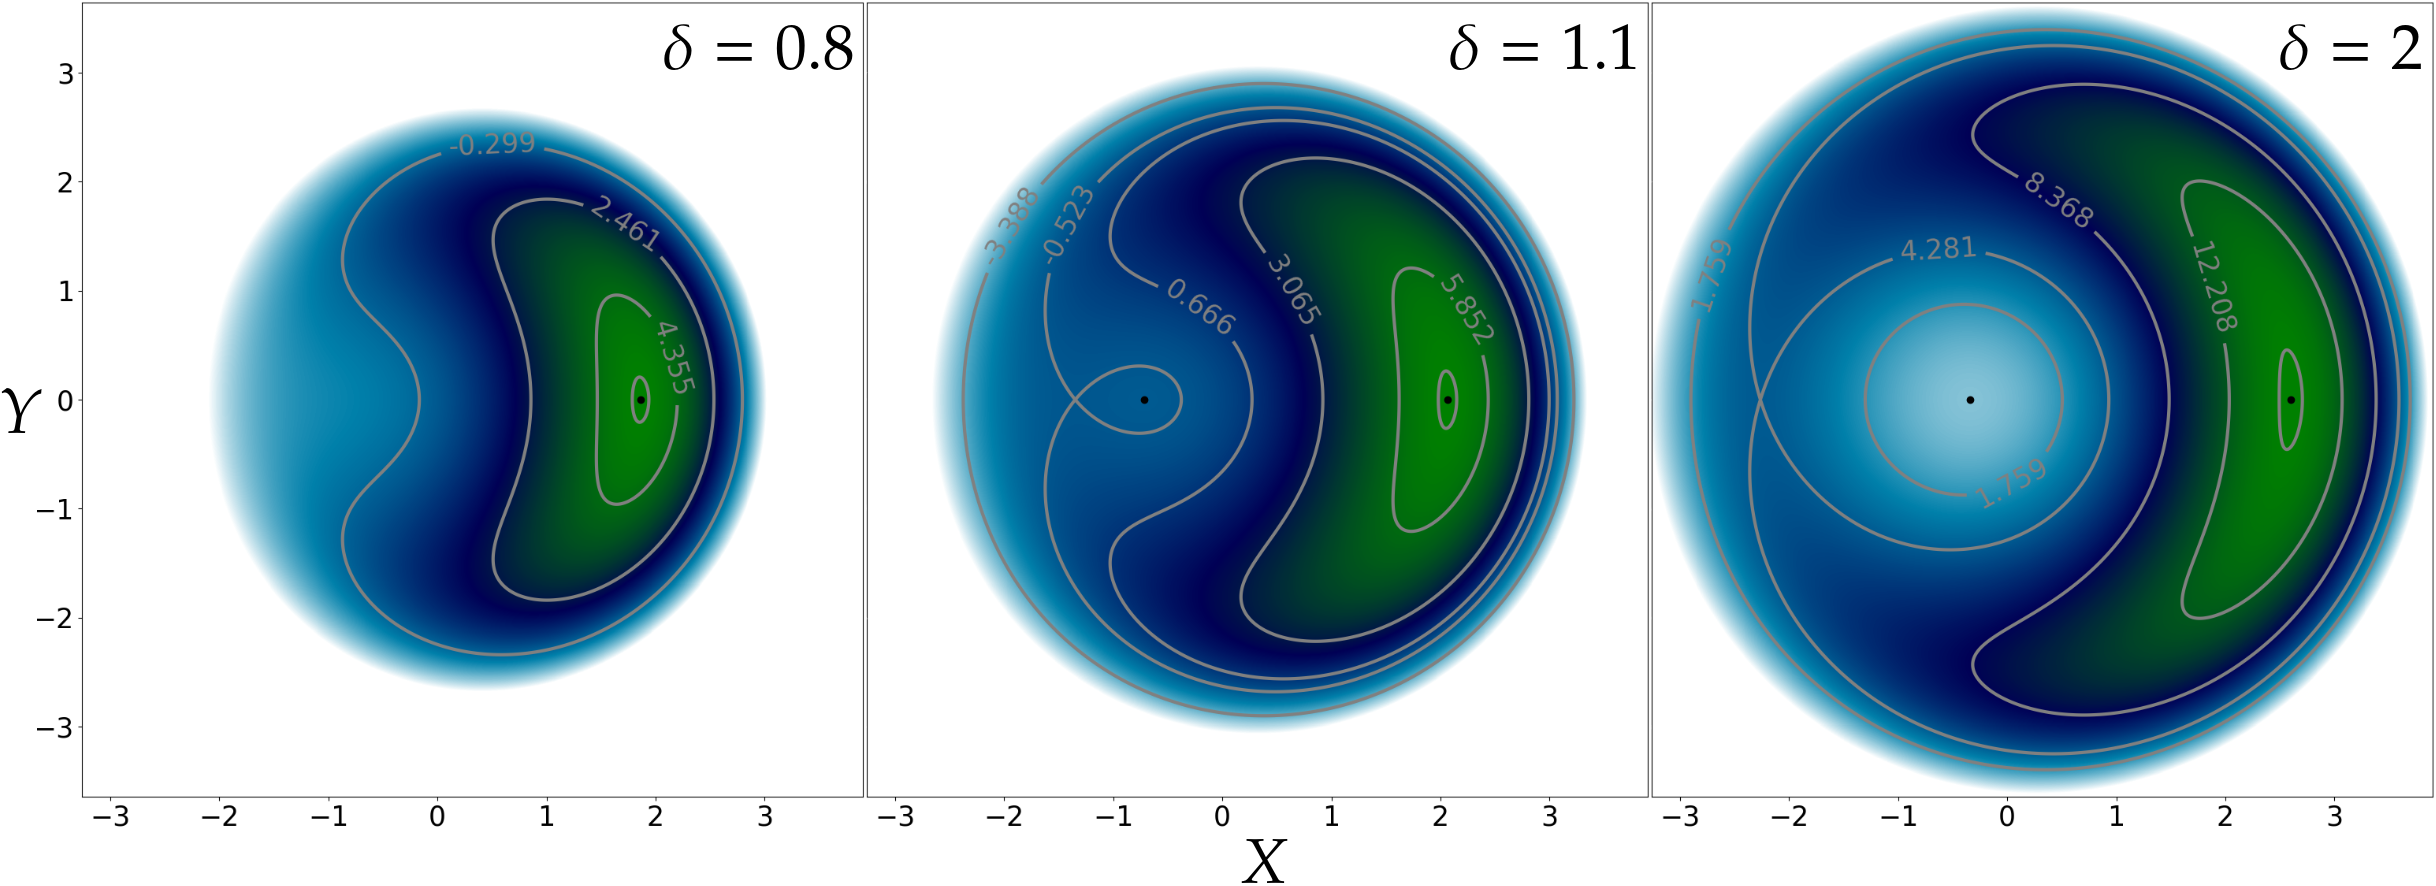
\includegraphics[width=\linewidth]{../img/PhaseSpaceSFM.png}
	\caption{Phase Space of the Hamiltonian (\ref{eq:XY_1param}) for $\delta\in\left\lbrace0.8,1.1,2\right\rbrace$. Elliptic fixed points are shown with a black point, whereas the hyperbolic fixed point is identified as the intersection of a level curve (the separatrix) with itself.}\label{fig:PhaseSpaceSFM}
\end{figure}
However, the canonical form can be recovered by merely rescaling time. Writing $\tau=\omega t/K$, we obtain $d\Sigma/d\tau=-\partial\amalg/\partial\sigma$ and $d\sigma/d\tau=\partial\amalg/\partial\Sigma$. Since \smash{$R=\OO\left(e_j^2\right)$} and \smash{$\beta/\gamma=\OO\left(m_0/m_j\right)$}, the new action $\Sigma$ has order of magnitude \smash{$\Sigma=\OO\left(e_j^2\right)\OO\left(m_0/m_j\right)^{2/3}$}. Defining the last parameter $\delta$ as
\begin{equation}
	\delta=\alpha\left(\frac{4}{27\beta\gamma^2}\right)^{1/3},
\end{equation}
the one-parameter and one-degree-of-freedom Hamiltonian of the second fundamental model of resonance reads
\begin{equation}\label{eq:SFM_polar}
	\amalg(\Sigma;\sigma)=3\delta\Sigma-\Sigma^2+2\sqrt{2\Sigma}\cos\sigma.
\end{equation}
Using the cartesian canonical coordinates
\begin{equation}
	X=\sqrt{2\Sigma}\cos\sigma,\;\;\;Y=\sqrt{2\Sigma}\sin\sigma,
\end{equation}
the Hamiltonian is written
\begin{equation}\label{eq:XY_1param}
	\amalg(X;Y)=\frac{3}{2}\delta\left(X^2+Y^2\right)-\frac{1}{4}\left(X^2+Y^2\right)^2+2X,
\end{equation}
or equivalently
\begin{equation}
	\amalg(X;Y)=2X-\frac{1}{4}\left(X^2+Y^2-3\delta\right)^2.
\end{equation}
The equilibria of $\amalg$ are located at $Y=0$ and $X$ the roots of
\begin{equation}
	X^3-3\delta X-2=0.
\end{equation}
The equilibrium values of $X$ are then
\begin{equation}
	\begin{split}
		&X_\text{eq}\in\left\lbrace u+v,\;\;ju+j^2v,\;\;j^2u+jv\right\rbrace,\text{where}\\
		&u=\left(1+\sqrt{1-\delta^3}\right)^{1/3},\\
		&v=\left(1-\sqrt{1-\delta^3}\right)^{1/3},
	\end{split}
\end{equation}
and $j=\exp(2i\pi/3)$. With the constraint that $X_\text{eq}$ is a real number, there is a bifurcation at $\delta=1$. When $\delta<1$, only one (elliptic) fixed point exists, whereas for $\delta>1$, three fixed points exist, one of them being hyperbolic from which a separatrix emanates and defines the mathematical resonance. In Fig. \ref{fig:PhaseSpaceSFM}, I plot the phase space of the Hamiltonian (\ref{eq:XY_1param}) for different values of $\delta$, showing the bifurcation at $\delta=1$. By linearizing the equations of motions in the vicinity of the fixed points, it can be shown that a fixed point is hyperbolic if, and only if, $\delta<X^2<3\delta$. 

\section{Explicit expression of the transformations towards one degree of freedom}\label{sec:first_integrals}

Working around the transformations of Sect. \ref{sec:1dof}, the variable $R$ reads
\begin{equation}
	R=\frac{f_1^2C_1d_1+f_2^2C_2d_2+2f_1f_2\sqrt{C_1d_1C_2d_2}\cos(\sigma_1-\sigma_2)}{f_1^2C_1+f_2^2C_2},
\end{equation}
whereas the first integral $S$ is given by
\begin{equation}
	S=\frac{f_1^2C_1d_2+f_2^2C_2d_1-2f_1f_2\sqrt{C_1d_1C_2d_2}\cos(\sigma_1-\sigma_2)}{f_1^2C_1+f_2^2C_2}.
\end{equation}
Using the equations of motions $\dot{d}_j=-\partial\Ham/\partial\sigma_j$ and $\dot{\sigma}_j=\partial\Ham/\partial d_j$ derived from the Hamiltonian $\Ham_K+\Ham_P$ given by Eqs. (\ref{eq:Hp_sigma_d}) and (\ref{final_Keplerian}), I verified that,
\begin{equation}
	\frac{dS}{dt}=\left\lbrace\Ham,S\right\rbrace=\drond{S}{d_1}\dot{d}_1+\drond{S}{d_2}\dot{d}_2+\drond{S}{\sigma_1}\dot{\sigma}_1+\drond{S}{\sigma_2}\dot{\sigma}_2=0,
\end{equation}
proving in another way that $S$ is indeed a conserved quantity. If $S$ is a conserved quantity, then so is $\Upsilon$, defined as
\begin{equation}
	\Upsilon=-2\frac{f_1^2C_1+f_2^2C_2}{f_1f_2}S.
\end{equation}
Using the relations \smash{$\sqrt{2C_jd_j}=e_j+\OO(e_j^3)$} and $\sigma_1-\sigma_2=\varpi_2-\varpi_1$, and the ratio
\begin{equation}
	\frac{e_{1,\text{eq}}}{e_{2,\text{eq}}}=\frac{f_1}{-f_2}\frac{m_2}{m_1}\left(\frac{p+1}{p}\right)^{1/3},
\end{equation}
between the equilibrium values of $e_j$ at the fixed point (the one that exists for all values of $\delta$), $\Upsilon$ can be written
\begin{equation}
	\Upsilon=\frac{e_{2,\text{eq}}}{e_{1,\text{eq}}}e_1^2+\frac{e_{1,\text{eq}}}{e_{2,\text{eq}}}e_2^2+2e_1e_2\cos(\varpi_1-\varpi_2).
\end{equation}
This gives, for resonances $1:2$ to $5:6$, respectively,
\begin{equation}
	\begin{split}
		&\Upsilon_{1:2}=0.28561\frac{m_1}{m_2}e_1^2+3.50132\frac{m_2}{m_1}e_2^2+2e_1e_2\cos(\varpi_1-\varpi_2),\\
		&\Upsilon_{2:3}=1.07148\frac{m_1}{m_2}e_1^2+0.93329\frac{m_2}{m_1}e_2^2+2e_1e_2\cos(\varpi_1-\varpi_2),\\
		&\Upsilon_{3:4}=1.05021\frac{m_1}{m_2}e_1^2+0.95219\frac{m_2}{m_1}e_2^2+2e_1e_2\cos(\varpi_1-\varpi_2),\\
		&\Upsilon_{4:5}=1.03873\frac{m_1}{m_2}e_1^2+0.96271\frac{m_2}{m_1}e_2^2+2e_1e_2\cos(\varpi_1-\varpi_2),\\
		&\Upsilon_{5:6}=1.03154\frac{m_1}{m_2}e_1^2+0.96943\frac{m_2}{m_1}e_2^2+2e_1e_2\cos(\varpi_1-\varpi_2).
	\end{split}
\end{equation}

%\singlespacing

%\appendix
%\include{Chapters/append/demo_love}
%\include{Chapters/append/coefficients_H4}
%\include{Chapters/append/differential_system}
%\include{Appendix/appB_AMDstab}
%\include{Appendix/appC_MMR}
%\include{Appendix/appD_Hill}
%\include{Appendix/appE_Integ}


\printbibliography[heading=bibintoc]
%\printbibliography[type=book]
\end{document}
